
\documentclass{article}
\usepackage{ragged2e} 
\usepackage{graphicx} % Required for inserting images
% Document dependencies
\usepackage[utf8]{inputenc}
\usepackage[square,sort,comma,numbers]{natbib}
\bibliographystyle{agsm}
\bibpunct{(}{)}{;}{a}{,}{,}
\usepackage{graphicx, adjustbox, rotating}
\usepackage{booktabs, url}
\usepackage{comment}
\usepackage{float}
\usepackage{pdflscape}
\usepackage{caption, subcaption}
\usepackage[margin=1in]{geometry} %margins
\usepackage[colorlinks = true, urlcolor = blue, linkcolor = blue, citecolor = blue]{hyperref}
\usepackage[parfill]{parskip} % first line skip 
\setlength{\parindent}{15pt} %for paragraph indent
\usepackage{indentfirst} %for first paragraph indent
\usepackage{setspace} %line spacing
 \usepackage{pdfpages}

\DeclareGraphicsExtensions{.pdf,.png,.jpg}
\pdfgentounicode=1

\title{The Effects of 287(g) Agreements on Immigrant's Mobility Decisions}
\author{Mena Kiser}
\date{\today}

\begin{document}
\doublespacing
\maketitle

\begin{abstract}
    287(g) agreements create partnerships between state and local agencies and ICE, allowing for deputized officers to perform some of ICE duties; this program led to deportations of immigrants of Hispanic origin burgeoning between 2011-2014. Out of fear of racial discrimination, Hispanic non-citizens may be more prone to moving out of counties with active 287(g) agreements. I explore this through a staggered difference-in-difference design evaluating the effect of living in a county with an active 287(g) agreement and being part of the population targeted by this policy compared to similar citizens in similar areas (identified through propensity score matching) without an active agreement. 
\end{abstract}

%\section{Introduction}

\section{287(g) Agreements}
The 287(g) program establishes partnerships between state and local enforcement agencies (LEAs) and ICE for local officers to exercise ICE duties to some extent. LEAs can voluntarily request participation in the program and ICE ultimately decides which agencie are included in the program and enters negotiation for a Memorandum of Agreement (MOA). MOAs are negotiated between DHS and LEAs and supervised by ICE; they establish delegation of authority to a determined number of officers. After an agreement expires, DHS is not obligated to renew it. Not all agreements include a specific expiration date, and once an agreement is entered into, it may be terminated at any time by either party.

This policy was officially enacted in 1996 as part of the Illegal Immigration Reform and Immigrant Responsibility Act (IIRIRA); however, no agencies joined the program until 2002 (Figure \ref{fig:timeline}). In 2008, ICE created a standard template for MOA, simplifying the process for LEAs to enroll. Between 2006 and 2009, at least 56 agencies joined the program. In September of 2025, DHS reported over 1,000 current MOAs, most of which were entered starting 2019.

This program can take three different models (and hybrids of these) based on the needs, capacity, and interest of the agency and ICE: 
\begin{enumerate}
    \item Jail Enforcement: LEA officers can interrogate and place detainers (requests to maintain in custody for up to 48 hours) for suspected noncitizens who have been arrested. This model has been available since its first enactment.
    \item Task Force: LEA officers can interrogate and arrest suspected noncitizens that they encountered in their daily activities. This model was available from its enactment until rescinded in December 2012, after which jail enforcement contracts were not renewed. In January 2025, this model was reinstated.  %https://www.ice.gov/news/releases/fy-2012-ice-announces-year-end-removal-numbers-highlights-focus-key-priorities-and
    \item Warrant Service Officer (WSO): LEA officers receive ICE training to execute immigration warrants. This model was first introduced in May 2019.
\end{enumerate}

Though this program has been in effect since its first enactment, changes in recruiting, funding, and DHS priorities for identifying undocumented immigrants may change the program's intensity.

While 287(g) agreements were in effect, other enforcement or (deferrement of enforcement) programs were enacted:
\begin{itemize}
    \item[a.] \textit{Secure Communities (SC)}
\end{itemize}


The most closely related program was Secure Communities, first effective in 2008. This policy established biometric information sharing between local LEAs and federal agencies for the detection of undocumented immigrants upon local detention. The program rolled out on a county-by-county basis from 2008 to 2014—the staggered release was due to technology barriers—until all U.S. counties were covered. Counties could not opt-in/out but LEAs had discretion to determine which detainers to honor. Currently, all counties should have access to this biometric information sharing system. On November 2014, the Secure Communities program was replaced by the Priority Enforcement Program (PEP). Under PEP, detainers, requests for transfer, or requests for notifications are issued to immigrants of immigration enforcement priority, who have participated in gang activity, or who pose a danger to national security. In January 2017, the Secure Communities program was reinstated. East et al. (\citeyear{east2023}) exploits the staggered nature of SC rollout identifying a decrease in employment and income levels for the likely undocumented male immigrants from X year to Y year. This study also evaluates the effect of 287(g) agreements in the localities of interest finding negative effects in labor market outcomes. This policy most closely resembles the jail enforcement modality of 287(g) agreements. To separate county differential effect of 287(g) program from SC, we focus on the 2013-2019 period avoiding overlapping with the SC rollout.


\begin{itemize}
    \item[b.] \textit{Deferred Action for Childhood Arrivals (DACA)}
\end{itemize}

In June 2012, Deferred Action for Childhood Arrivals (DACA) was introduced providing legal status to unauthorized immigrants who had arrived in the United States as children. DACA provided deportation deferral and Employment Authorization Document, which allowed them to legally work in the US. Eligibility for DACA was determined by five main criteria:  1) U.S. arrival before their sixteenth birthday; 2) continuously lived in the U.S. since June 2007; 3) under age of 31 by June 2012; 4) high school (or equivalent) completion of or current enrollment in school; and 5) they have not been convicted of a a felony or significant misdemeanor. The take-up of DACA was both large and immediate. Kiser and Wilson (2025) provide evidence of the positive effect of DACA eligibility on the likelihood of moving relative to those barely ineligible upon its enactment, as the policy provided them with tools to make longer-lasting economic decisions. To rule out mobility differentials, I restrict the sample to immigrants that arrived in the U.S. after 2007, making them ineligible for DACA.


\section{Data}
The main datasets used in this paper come from the ICE websites,  Syracus University Transactional Records Access Clearinghouse (TRAC), and from the American Community Survey (ACS). 

Through the Internet Archive's Wayback Machine, I can extract snapshots from ICE websites listing LEAs with current 287(g) agreements starting. These lists are retrievable starting in 2011. All lists include the name of the agency, the date it was signed, and the type of agreement entered. For each year, I can obtain a minimum of 3 snapshots from different days in different months, as seen in Table \ref{tab:retrievals}. Having access to multiple observations within a year allows me to identify the dates when agreements were terminated, as indicated by their absence from subsequent retrievals. I match agencies to their local geographic area using the name of the agency, e.g. Jackson County Sheriff’s Office (KS) is assigned Jackson County, KS. \footnote{I'm in the process of assigning geographic areas using Law Enforcement Agency Identifiers Crosswalk (2012).} From 2013 to 2019, I can identify 123 distinct agencies with some active agreement mapping to 70 distinct counties. at any point between 2014 and 2019. 

Exposure is defined based on the number of months a county had some active agreement and the coverage of the agreement (calculated using population). In other words, as shown in Equation \ref{eq:exposure} exposure for a county ($c$) in year ($y$) is defined by the yearly average of MOA in a jurisdiction ($j$) active on days ($d$) weighted by coverage of jurisdiction to county using 2010 population estimates.

\begin{equation}
\label{eq:exposure}
    exposure_{cy} = \sum_{d=1}^{365} \sum_{j=1} ^{J} \frac{MOA_{dj}}{365} * \frac{pop_{j}}{pop_{c}}
\end{equation}

Exposure can span from 0-1 based on the number of agencies with active agreements in a locality. In a given year, an exposure of 0, signals there was no active 287(g) agreement during year. An exposure between 0 and 1, signals there was an agreement at some point during the year that was not active during the whole month or did not cover the full county. An exposure of 1, signals there is an active agreement during the whole year and covering the whole county. A exposure over 1, means there are multiple agreements in the area, for instance, the county jail and the sheriff's department can both have active agreements; however, we do not observe exposure greater than 1 during this sample. This setup assumes a county with multiple agreements is different from counties with only one agreement.

I obtain details on the demographics of those targeted by 287(g) from the Transactional Records Access Clearinghouse \citep{trac24}, an organization founded by the Syracuse University that gathers and distributes immigration statistics obtained from government agencies through the Freedom of Information Act (FOIA). From reports on ICE removals initiated with a 287(g) Program apprehension, we can see that 67\% of the deportees were of ages 18--39, 97\% had citizenship in a Latin American country, and 96\% were male. 

Individual characteristics are extracted from the 2013-2019 American Community Survey (ACS), obtained through the Integrated Public Use Microdata Series (IPUMS) \citep{data:acs}. The ACS is a yearly cross-sectional, one percent, annual survey of households in the United States. Through this survey we can identify foreign-born respondents using place of birth and citizenship status; however, this survey does not ask about current legal status or status at entry. Following existing work imputing a citizenship status, I define the population targeted by this program as those fitting the predominant demographics of removed immigrants and those likely to be undocumented: ages 18-29, Hispanic, foreign-born, non-citizen, male, low-skill (high school degree or less). I further restrict to those with US arrival after 2007 to rule out DACA eligibility and those not currently married to rule out citizenship eligibility through their spouse and as the unmarried may be more responsive to policy shocks.\footnote{A more elegant design would use evidence from a survey describing characteristics of the undocumented.} I also restrict to those with 10 years or less in the country as they may also be more responsive. In Table \ref{tab:sumstat}, we can observe characteristics of the targeted population across level of exposure.

The ACS includes an individual's state and county of current residence and previous year residence. This source also provides  place of work county, commuting time, current occupation, industry, earnings, and more which will help us understand other effects of this policy.


\section{Empirical design}
To identify the effects of this policy, I use a difference-in-difference design interacting being part of the target population and exposure, as shown in Equation \ref{eq:did}. However, as treatment is quite unbalanced, I use a propensity score matching to re-weight untreated counties. Through a logit estimation regressing on a county's share of targeted population, low skill population, foreign population, young population, total population, mean income, house price (either rent or mortgage), and being a predominantly red state. The predicted exposure score along with the original non-zero scores are applied to the untreated. 
As the cross-sectional data from ACS uses probability weights, I multiply these by the propensity score obtained and apply this for all analysis. In Table \ref{tab:sumstat}, we can observe how relevant characteristics for the treated and untreated groups changes when applying the propensity score weights.
\begin{equation}
    \label{eq:did}
    in-migration_{icy} = \beta_{0} + \beta_{1}exposure_{cy}*targeted_{i} +  \beta_{2}exposure_{cy} + \beta_{3}targeted_{i} + \beta_{42}W_{y} + \beta_{53}Z_{c} + \epsilon_{cy} 
\end{equation}

To first test the parallel trends assumption, we can evaluate the effect of exposure on migration decisions, following Equation \ref{eq:reg1}, in which in--migration can take any move (including within county), moving counties, and moving states. I include the results for this estimation in Table \ref{tab:regtp}. We can see that in the targeted population, 287(g) exposure increases mobility within county, across counties, and across states, with a higher significance level at county level. These results become stronger and more significant when applying propensity weights. In the placebo population, we observe mostly negative effects and not-statistically significant effects of 287(g) programs in mobility.
\begin{equation}
    \label{eq:reg1}
    in-migration_{icy} = \beta_{0} + \beta_{1}exposure_{cy} +  \beta_{42}W_{y} + \beta_{53}Z_{c} + \epsilon_{cy} 
\end{equation}

These results suggest there are differential effects in migration for the non-citizen targeted population, distinct from similar citizens. However, the direction of the effect has the opposite of the sign expected. I initially hypothesized that areas in which 287(g) is currently enacted, targeted immigrants would be less likely to move to areas where these agreements have been recently enacted. We are seeing that areas with active MOAs are more likely to have newcomers from the targeted population. A possible explanation for this, is that deporting immigrants in this group creates job vacancies and may potentially increase wages if demand for low-skilled Hispanic workers is not met, thus immigrants move to these areas in pursue of better economic opportunities. To validate this new hypothesis we must also check economic outcomes.

\begin{comment}

in migration: previous year is different from the current year
\begin{equation}
    in-migration_{icy} = \beta_{0} + \beta_{1}exposure_{cy}*targeted_{i} +  \beta_{2}exposure_{cy} + \beta_{3}targeted_{i} + \beta_{42}W_{y} + \beta_{53}Z_{c} + \epsilon_{cy} 
\end{equation}

out migration 
\begin{equation}
    out-migration_{ic'y'} = \beta'_{0} + \beta'_{1}exposure_{c'y'}*targeted_{i} + \beta'_{2}exposure_{c'y'} + \beta'_{3}targeted_{i} + \beta'_{42}W_{y'} + \beta'_{43}Z_{c'} + \epsilon_{c'y'} 
\end{equation}
\end{comment}

\bibliography{bib_287.bib}

\newpage
\section{Tables and Figures}

\begin{table}[h]
\centering
\caption{Retrievals of active Memorandum of Agreements}
\label{tab:retrievals}
\adjustbox{ width=0.4\linewidth}{
    \begin{tabular}{lccc}
\toprule
\toprule
 & \multicolumn{3}{c}{Distinct retrivals} \\
 Year & Days & Months & LEAs \\
\midrule 
2011 & 3 & 3 & 71 \\
2012 & 37 & 8 & 68 \\
2013 & 6 & 6 & 57 \\
2014 & 3 & 3 & 37 \\
2015 & 16 & 9 & 34 \\
2016 & 13 & 8 & 34 \\
2017 & 125 & 12 & 62 \\
2018 & 306 & 12 & 79 \\
2019 & 332 & 12 & 94 \\
\bottomrule
\bottomrule
\end{tabular}
}
\end{table}

\justifying
\
\begin{spacing}{1}
\begin{footnotesize}
\noindent \textit{Notes:} This table quantifies the number of retrievals from distinctive days, months, and pertaining different Local Enforcement Agencies (LEAs).
\end{footnotesize}
\end{spacing}


\newpage
\begin{landscape}
\begin{table}[h]
\centering
\caption{Summary statistics by exposure and target group}
\label{fig:timeline}
\adjustbox{ width=\linewidth}{
    \begin{tabular}{lcccccccc}
\toprule
\toprule
 & & & & & \multicolumn{4}{c}{Propensity score weighting} \\
 & \multicolumn{2}{c}{Targeted population} & \multicolumn{2}{c}{Hispanic citizens} & \multicolumn{2}{c}{Targeted population} & \multicolumn{2}{c}{Hispanic citizens}  \\
 & Exposure=0 & Exposure$>$0 & Exposure=0 & Exposure$>$0 & Exposure=0 & Exposure$>$0 & Exposure=0 & Exposure$>$0 \\
 & (1) & (2) & (3) & (4) & (5) & (6) & (7) & (8) \\
\midrule 
 Male  & 1.00 & 1.00 & 1.00 & 1.00 & 1.00 & 1.00 & 1.00 & 1.00\\
 Age  & 26.36 & 26.32 & 25.25 & 24.73 & 26.59 & 26.38 & 25.35 & 24.78\\
 Exposure  & 0.00 & 0.46 & 0.00 & 0.44 & 0.00 & 0.42 & 0.00 & 0.41\\
 High School  & 0.46 & 0.43 & 0.76 & 0.75 & 0.44 & 0.42 & 0.77 & 0.74\\
 Any move  & 0.25 & 0.31 & 0.16 & 0.16 & 0.24 & 0.30 & 0.13 & 0.15\\
 Moved county  & 0.12 & 0.14 & 0.05 & 0.04 & 0.11 & 0.13 & 0.03 & 0.03\\
 Moved state  & 0.09 & 0.12 & 0.02 & 0.02 & 0.08 & 0.12 & 0.01 & 0.02\\
 Married  & 0.00 & 0.00 & 0.00 & 0.00 & 0.00 & 0.00 & 0.00 & 0.00\\
 Never married  & 0.94 & 0.93 & 0.94 & 0.95 & 0.94 & 0.93 & 0.95 & 0.95\\
 Number of children  & 0.23 & 0.25 & 0.23 & 0.21 & 0.24 & 0.26 & 0.21 & 0.21\\
 Employed  & 0.84 & 0.87 & 0.64 & 0.66 & 0.86 & 0.87 & 0.65 & 0.64\\
 Weeks worked  & 41.49 & 42.01 & 33.59 & 36.78 & 42.11 & 42.45 & 34.29 & 36.66\\
 Usual weekly hours worked  & 35.31 & 36.17 & 26.80 & 27.54 & 35.99 & 36.03 & 27.17 & 27.07\\
 Wage income  & 22,858.94 & 21,025.92 & 22,884.53 & 21,599.17 & 23,481.98 & 20,363.06 & 23,771.22 & 21,419.30\\
 Owns a home  & 0.16 & 0.14 & 0.47 & 0.47 & 0.15 & 0.13 & 0.48 & 0.47\\
 Rent price  & 1,077.29 & 883.61 & 1,002.44 & 1,011.13 & 1,086.20 & 857.90 & 1,081.54 & 989.07\\
 Mortgage price  & 931.81 & 695.44 & 918.96 & 886.21 & 989.62 & 747.43 & 961.93 & 887.72\\
 Sample size  & 9,107.00 & 2,860.00 & 69,284.00 & 21,022.00 & 9,107.00 & 2,860.00 & 69,284.00 & 21,022.00\\
\bottomrule
\bottomrule
\end{tabular}
}
\end{table}

\justifying
\begin{spacing}{1}
\begin{footnotesize}
\noindent \textit{Notes:} This table summarizes main characteristics by exposure and population type. Columns 1-2 and 5-6 restrict the sample to immigrants likely targeted by 287(g) agreements: foreign-born non-citizen, Hispanic, male, of ages 18-39, with High School degree or less, that immigrated after 2007, have been in the US for 10 years or less, and are not currently married. Columns 3-4 and 7-8 restricts the sample to comparable individuals, meeting all criteria from the targeted sample except they must be US-born citizens (thus no immigration time requirements). Odd-numbered columns restrict the sample to (untreated) zero exposure counties and even-numbered columns restrict the sample to non-zero exposure counties. Columns 1-4 apply probability weights as extracted from ACS, while columns 5-8 apply weights obtained from propensity score matching.
\end{footnotesize}
\end{spacing}
\end{landscape}




\newpage
\begin{table}[h]
\centering
\caption{Exposure to 287(g)  on targeted and placebo populations}
\label{tab:regtp}
\adjustbox{ width=0.7\linewidth}{
    \begin{tabular}{lcccc}
\toprule
\toprule
 & & & \multicolumn{2}{c}{Propensity weighting}  \\
 & Targeted & Placebo & Targeted & Placebo \\
 & (1) & (2)  & (3) & (4)  \\
\midrule 
 Any move & 0.0653** & -0.0088 & 0.0825*** & -0.0046 \\
 \textit{SE} & (0.0279) & (0.0081) & (0.0251) & (0.0071) \\
 \textit{R2} & 0.0781 & 0.0400 & 0.0671 & 0.0306  \\
 \textit{F-stat} & 5.4634 & 1.1810 & 10.8307 & 0.4240  \\
\\
 Move county & 0.0592*** & -0.0054 & 0.0744*** & -0.0015 \\
 \textit{SE} & (0.0206) & (0.0047) & (0.0189) & (0.0035) \\
 \textit{R2} & 0.0732 & 0.0352 & 0.0630 & 0.0221  \\
 \textit{F-stat} & 8.2512 & 1.3422 & 15.4223 & 0.1831  \\
\\
 Move state & 0.0450** & -0.0008 & 0.0573*** & 0.0014 \\
 \textit{SE} & (0.0190) & (0.0025) & (0.0187) & (0.0023) \\
 \textit{R2} & 0.0715 & 0.0287 & 0.0587 & 0.0156  \\
 \textit{F-stat} & 5.5966 & 0.1104 & 9.3338 & 0.3534  \\
\\
Sample Size  & 11,925  & 11,925  & 11,925  & 11,925 \\
\bottomrule
\bottomrule
\end{tabular}
}
\end{table}

\justifying
\begin{spacing}{1}
\begin{footnotesize}
\noindent \textit{Notes:} This table compares the effect of exposure to a 287(g) program across targeted population and a placebo population defined by those who meet all criteria of targeted population except they are US-born citizens. Columns 3-4 adjust the ACS weights by the propensity score. Each cell represents a different regression. Standard errors are set at the county-year level and county and year fixed effects are absorbed. p $<$ 0.01 ***, p $<$ 0.05 **, p $<$0.1 *. 

\end{footnotesize}
\end{spacing}



\newpage
\begin{landscape}
    
\begin{figure}[h]
\centering
\caption{Timeline of the evolution of 287(g) agreements}
\label{tab:regtp}
\adjustbox{ width=\linewidth}{
    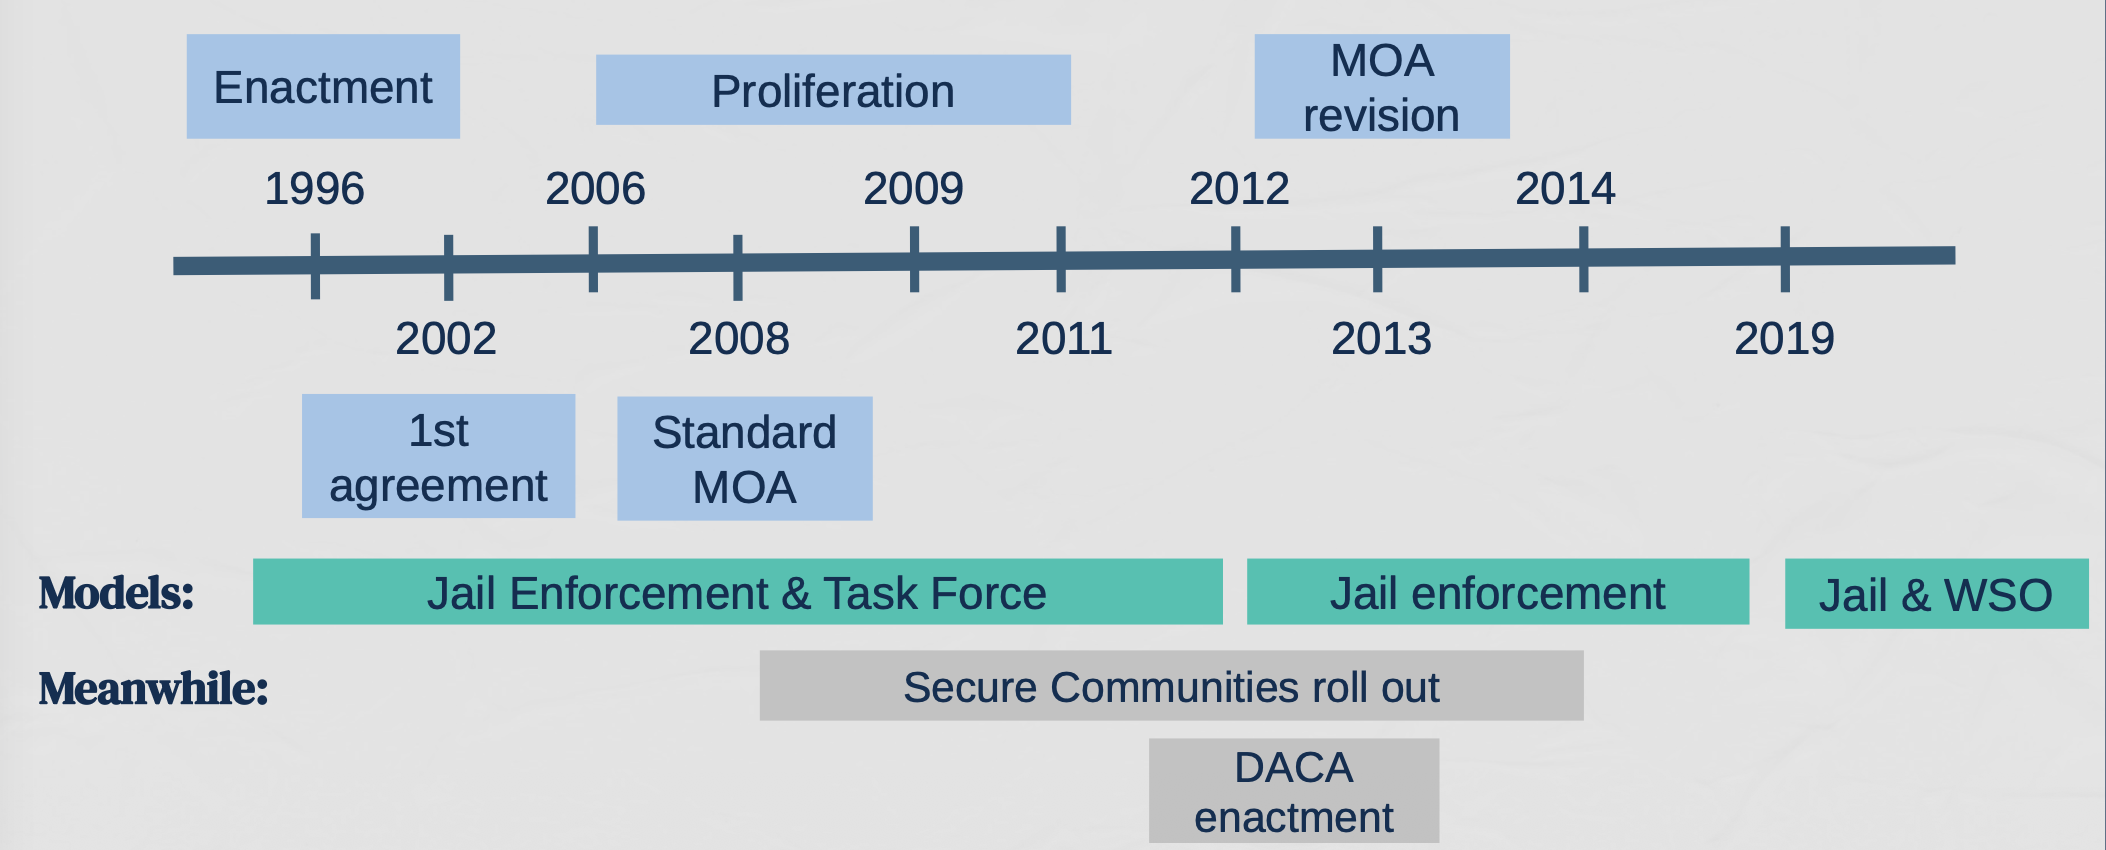
\includegraphics{output/timeline.png}
}
\end{figure}

\justifying
\begin{spacing}{1}
\begin{footnotesize}
\noindent \textit{Notes: This timeline includes events relevant to the current panorama of the 287(g) program.}

\end{footnotesize}
\end{spacing}

\end{landscape}

\end{document}
